\documentclass[10pt,a4paper]{article}
\usepackage[UTF8,fontset = windows]{ctex}
\setCJKmainfont[BoldFont=黑体,ItalicFont=楷体]{华文中宋}
\usepackage{amssymb,amsmath,amsfonts,amsthm,mathrsfs,dsfont,graphicx}
\usepackage{ifthen,indentfirst,enumerate,color,titletoc}
\usepackage{tikz}
\usepackage{multicol}
\usepackage{makecell}
\usepackage{longtable}
\usetikzlibrary{arrows,calc,intersections,patterns,decorations.pathreplacing,3d,angles,quotes}
\usepackage[bf,small,indentafter,pagestyles]{titlesec}
\usepackage[top=1in, bottom=1in,left=0.8in,right=0.8in]{geometry}
\renewcommand{\baselinestretch}{1.65}
\newtheorem{defi}{定义~}
\newtheorem{eg}{例~}
\newtheorem{ex}{~}
\newtheorem{rem}{注~}
\newtheorem{thm}{定理~}
\newtheorem{coro}{推论~}
\newtheorem{axiom}{公理~}
\newtheorem{prop}{性质~}
\newcommand{\blank}[1]{\underline{\hbox to #1pt{}}}
\newcommand{\bracket}[1]{(\hbox to #1pt{})}
\newcommand{\onech}[4]{\par\begin{tabular}{p{.9\textwidth}}
A.~#1\\
B.~#2\\
C.~#3\\
D.~#4
\end{tabular}}
\newcommand{\twoch}[4]{\par\begin{tabular}{p{.46\textwidth}p{.46\textwidth}}
A.~#1& B.~#2\\
C.~#3& D.~#4
\end{tabular}}
\newcommand{\vartwoch}[4]{\par\begin{tabular}{p{.46\textwidth}p{.46\textwidth}}
(1)~#1& (2)~#2\\
(3)~#3& (4)~#4
\end{tabular}}
\newcommand{\fourch}[4]{\par\begin{tabular}{p{.23\textwidth}p{.23\textwidth}p{.23\textwidth}p{.23\textwidth}}
A.~#1 &B.~#2& C.~#3& D.~#4
\end{tabular}}
\newcommand{\varfourch}[4]{\par\begin{tabular}{p{.23\textwidth}p{.23\textwidth}p{.23\textwidth}p{.23\textwidth}}
(1)~#1 &(2)~#2& (3)~#3& (4)~#4
\end{tabular}}
\begin{document}
\begin{enumerate}[1.]
\item 判断下列各组对象能否组成集合. 若能组成集合, 指出是有限集还是无限集; 若不能组成集合, 请说明理由.\\
(1) 上海市现有各区的名称;\\
(2) 末位是$3$的自然数;\\
(3) 比较大的苹果.
\item 用符号``$\in$''或``$\not\in$''填空:\\
(1) $\dfrac12$\blank{50}$\mathbf{N}$;\\
(2) $5$\blank{50}$\mathbf{Z}$;\\
(3) $-2$\blank{50}$\mathbf{Q}$;\\
(4) $\pi$\blank{50}$\mathbf{R}$. 
\item 用列举法表示下列集合:\\
(1) 能整除$10$的所有正整数组成的集合;\\
(2) 绝对值小于$4$的所有整数组成的集合.
\item 用描述法表示下列集合:\\
(1) 全体偶数组成的集合;\\
(2) 平面直角坐标系中$x$轴上所有点组成的集合.
\item 用区间表示下列集合:\\
(1) $\{x|-1<x\le 5\}$;\\
(2) 不等式$-2x>6$的所有解组成的集合. 
\item 判断下列说法是否正确, 并简要说明理由:\\
(1) 若$a\in A$且$A\subseteq B$, 则$a\in B$;\\
(2) 若$A\subseteq B$且$A\subseteq C$, 则$B=C$;\\
(3) 若$A\subset B$且$B\subseteq C$, 则$A\subset C$.
\item 用符号``$\supset$''``$=$''或``$\subset$''填空:\\
(1) $\{a\}$\blank{50}$\{a, b, c\}$;\\
(2) $\{a, b, c\}$\blank{50}$\{a, c\}$;\\
(3) $\{1, 2\}$\blank{50}$\{x|x^2-3x+2=0\}$.
\item 写出所有满足$\{a\}\subset M\subset \{a, b, c, d\}$的集合$M$.
\item 设$A$为全集$U$的任一子集, 则
(1) $\overline{\overline{A}}=$\blank{50}; (A表示A的补集A的补集)\\
(2) $A\cap \overline A=$\blank{50};\\
(3) $A\cup \overline A=$\blank{50}.
\item 已知全集为$\mathbf{R}$, 集合$A=\{x|-2<x\le 1\}$. 求$A$.
\item 已知集合$A=\{1, 2, 3, 4, 5\}$, $B=\{2, 4, 6, 8\}$, $C=\{3, 4, 5, 6\}$. 求:\\
(1) $(A\cap B)\cup C$, $(A\cup C)\cap (B\cup C)$;\\
(2) $(A\cup B)\cap C$, $(A\cap C)\cup (B\cap C)$.
\item 举几个生活中的命题的例子, 并判断其真假.
\item 判断下列命题的真假, 并说明理由:\\
(1) 所有偶数都不是素数;\\
(2) $\{1\}$是$\{0, 1, 2\}$的真子集;\\
(3) $0$是$\{0, 1, 2\}$的真子集;\\
(4) 如果集合$A$是集合$B$的子集, 那么$B$不是$A$的子集.
\item 用``$\Rightarrow$''表示下列陈述句$\alpha$与$\beta$之间的推出关系:\\
(1) $\alpha: \triangle ABC$是等边三角形, $\beta: \triangle ABC$是轴对称图形;\\
(2) $\alpha: x^2=4$, $\beta: x=2$.
\item 已知$\alpha$: 四边形$ABCD$的两组对边分别平行, $\beta$: 四边形$ABCD$为矩形, $\gamma$: 四边形$ABCD$的两组对边分别相等. 用``充分非必要''``必要非充分''``充要''或``既非充分又非必要''填空:\\
(1) $\alpha$是$\beta$的\blank{50}条件;\\
(2) $\beta$是$\gamma$的\blank{50}条件;\\
(3) $\alpha$是$\gamma$的\blank{50}条件.
\item 设$\alpha: 1\le x<4$, $\beta: x<m$, $\alpha$是$\beta$的充分条件. 求实数$m$的取值范围.
\item 设$n\in \mathbf{Z}$. 证明: 若$n^3$是奇数, 则$n$是奇数.
\item 证明: 对于三个实数$a$、$b$、$c$, 若$a\ne c$, 则$a\ne b$或$b\ne c$. 
\item 设$a$、$b$、$c$、$d$是实数, 判断下列命题的真假, 并说明理由:\\
(1) 若$a^2=b^2$, 则$a=b$;\\
(2) 若$a(c^2+1)=b(c^2+1)$, 则$a=b$;\\
(3) 若$ab=0$, 则$a=0$或$b=0$;\\
(4) 若$\dfrac ac=\dfrac bd$, 且$c+d\ne 0$, 则$\dfrac{a+b}{c+d}=\dfrac ac$.
\item 设$a\in \mathbf{R}$, 求关于$x$的方程$ax=a^2+x-1$的解集.
\item 设$k\in \mathbf{R}$, 求关于$x$与$y$的二元一次方程组$\begin{cases}y=kx+1, \\ y=2kx+3 \end{cases}$的解集. 
\item 求一元二次方程$ax^2-4x+2=0$($a\ne 0$)的解集.
\item 已知方程$2x^2+4x-3=0$的两个根为$x_1$、$x_2$, 求下列各式的值:\\
(1) $x_1^2x_2+x_2^2x_1$;\\
(2) $\dfrac1{x_1}+\dfrac1{x_2}$;\\
(3) $x_1^2+x_2^2$;\\
(4) $x_1^3+x_2^3$. 
\item 设$a$、$b$、$c$、$d$为实数, 判断下列命题的真假, 并说明理由:\\
(1) 如果$a>b$, $c>d$, 那么$a+d>b+c$;\\
(2) 如果$ab>ac$, 那么$b>c$;\\
(3) 如果$a\ge b$且$a\le b$, 那么$a=b$;\\
(4) 如果$a>b$, $\dfrac 1c>\dfrac 1d$, 那么$ac>bd$;\\
(5) 如果$\dfrac ba>\dfrac dc$, 那么$bc>ad$.
\item 设$ab>0$, 求证: $a>b$是$\dfrac 1a<\dfrac 1b$的充要条件. 
\item 设$a$、$b$、$c$是实数, 判断下列命题的真假, 并说明理由.\\
(1) 如果$ac^2>bc^2$, 那么$a>b$;\\
(2) 如果$ab>c$, 那么$a>\dfrac cb$;\\
(3) 如果$a>b\ge 0$, 那么$\sqrt a>\sqrt b$.
\item 设$x$是实数, 比较$x^2+4$与$4x$的值的大小. 
\item 设$a\ne 1$, 解关于$x$的不等式: $ax<a^2+x-1$.
\item 填空题:\\
(1) $(x-2)(x+3)<0$的解集是\blank{50};\\
(2) $(2-x)(x+3)<0$的解集是\blank{50};\\
(3) $(x-2)(x+3)\ge 0$的解集是\blank{50}.
\item 求下列不等式的解集:\\
(1) $-8x\le 3x^2+4$;\\
(2) $-x^2<2x-4$. 
\item 解下列不等式:\\
(1) $x+2>-x^2$;\\
(2) $-x^2+3x-4>0$;\\
(3) $9x^2-6x+1>0$;\\
(4) $4x-x^2>4$;\\
(5) $2x^2+1\ge x$;\\
(6) $x^2+\dfrac 19\ge \dfrac 23x$.
\item 写出一个一元二次不等式, 使它的解集分别为:\\
(1) $(3-\sqrt 2, 3+\sqrt 2)$;\\
(2) $(-\infty, 3-\sqrt 2]\cup [3+\sqrt 2, +\infty)$;\\
(3) $\mathbf{R}$;\\
(4) $\varnothing$.
\item 求下列不等式组的解集:\\
(1) $\begin{cases} x^2-2x-3>0, \\ x-1>0; \end{cases}$\\
(2) $\begin{cases} x^2-2x-15\ge 0, \\ x^2-4x-12<0. \end{cases}$\\
\item 若关于$x$的不等式$x^2-x+m<0$的解集为$\varnothing$, 求实数$m$的取值范围.
\item 已知一元二次不等式$x^2-ax-b<0$的解集为$(2, 3)$, 求实数$a$、$b$的值及不等式$bx^2-ax-1>0$的解集.
\item 解下列不等式:\\
(1) $\dfrac{3-2x}{x-1}<0$;\\
(2) $\dfrac{2x-1}{x+2}\le 0$;\\
(3) $\dfrac{2x-1}{x-1}>2$;\\
(4) $\dfrac{4+x}{2+x}\ge 2$;\\
(5) $\dfrac{x-1}{x^2-4x+5}>1$;\\
(6) $\dfrac{4-x}{x^2+x+1}\le -1$. 
\item 解下列不等式:\\
(1) $|x+3|<4$;\\
(2) $|1-2x|>3$;\\
(3) $|2x-3|<3x-2$;\\
(4) $|x+1|+|x-4|>7$. 
\item 设$a$是正数, 求证: $a+1\ge 2\sqrt a$.
\item 证明: 若$x<0$, 则$x+\dfrac 1x\le -2$, 并指出等号成立的条件.
\item 用一根长为$l$的铁丝制成一个矩形框架. 当长和宽分别为多少时, 该框架的面积最大?
\item 在面积为$\pi$的圆中作一个内接矩形, 使它的面积最大. 求此矩形面积的最大值及此时矩形的各边长.  
\item 已知$a$、$b\in \mathbf{R}$. 求证: $|a+b| +|a-b| \ge 2|b|$.
\item 已知实数$a$、$b$满足$|a| <\dfrac 12$, $|b| <\dfrac 12$. 证明下列各式:\\
(1) $|a+b| <1$;\\
(2) $|a-b| <1$. 
\item 求$-\dfrac{32}{243}$的$5$次方根.
\item 求$9$的$4$次方根.
\item 求下列各根式的值:\\
(1) $\sqrt[5]{(-4)^5}$;\\
(2) $\sqrt[6]{(a-b)^6}$(其中$a<b$).
\item 求下列各式的值:\\
(1) $100^\frac 12$;\\
(2) $8^{-\frac23}$.
\item 用有理数指数幂的形式表示下列各式(其中$a>0$):\\
(1) $a^{\frac{10}3}\cdot \sqrt[5]{a^3}$;\\
(2) $\sqrt[3]{a\sqrt[3]{a}}$.
\item 化简下列各式:\\
(1) $(a^{3+\sqrt 3})^{3-\sqrt 3}$(其中$a>0$);\\
(2) $\dfrac{4a^{\frac 23}b^2}{(a^{\frac 16}b^{\frac 56})(-\dfrac 23 a^{\frac 12}b)}$(其中$a>0$, $b>0$).
\item 已知$0<a<1$, $s>0$. 求证: $0<a^s<1$.
\item 以下对数式中, 与指数式$5^x=6$等价的是\bracket{20}.
\fourch{$\log_56=x$}{$\log_5x=6$}{$\log_6x=5$}{$\log_x6=5$}
\item 求下列各式的值:\\
(1) $\log_525$;\\
(2) $\log_{\frac 13}27$;\\
(3) $\log_4\sqrt 2$;\\
(4) $2^{\log_23}$.
\item 求下列各式中$x$的值:\\
(1) $\log_4x=2$;\\
(2) $\log_x4=2$. 
\item 已知$A=\log_ax$, $B=\log_ay$($a>0$且$a\ne 1$). 用$A$及$B$表示下列各式:\\
(1) $\log_axy$;\\
(2) $\log_ax^2\sqrt y$.
\item 求下列各式的值:\\
(1) $\log_{15}3+\log_{15}5$;\\
(2) $\log_2\sqrt[3]{4}$;\\
(3) $\log_5\sqrt{10}-\dfrac 12\log_5250$.
\item 已知$\log_73=a$, $7^b=2$. 用$a$及$b$表示$\log_772$. 
\item 求下列各式的值:\\
(1) $\log_8\dfrac 14$;\\
(2) $\log_ab\cdot\log_bc\cdot\log_ca$($a$、$b$、$c$均为不等于$1$的正数);\\
(3) $3^{2+\log_94}$;\\
(4) $\dfrac{\log_52\times\log_79}{\log_5\dfrac 13\times\log_72}$.
\item 已知$\log_32=a$, 用$a$表示$\log_296$.
\item 设$a$、$b$是两个不等于$1$的正数, 求证: $\log_ba=\dfrac1{\log_ab}$.
\item 若幂函数$y=x^a$的图像经过点$(3, \sqrt 3)$, 求此幂函数的表达式.
\item 求下列函数的定义域, 并作出它们的大致图像:\\
(1) $y=x^{\frac 13}$;\\
(2) $y=x^{-\frac 12}$;\\
(3) $y=x^{\frac 43}$.
\item 若幂函数$y=x^{-m^2+2m+3}$($m$为整数)的定义域为$\mathbf{R}$, 求$m$的值.
\item (1) 已知函数$y=x^{\frac 23}$和$y=(x-1)^{\frac 23}$, 说明这两个函数图像之间的关系, 并在同一平面直角坐标系中作出它们的大致图像;\\
(2) 已知函数$y=x^{\frac 23}$和$y=x^{\frac 23}+1$, 说明这两个函数图像之间的关系, 并在同一平面直角坐标系中作出它们的大致图像.
\item 比较下列各题中两个数的大小:\\
(1) $2.5^{-3}$与$3.1^{-3}$;\\
(2) $1.7^{\frac 32}$与$1.6^{\frac 32}$.
\item 作出函数$y=\dfrac{-x-1}{x+2}$的大致图像.
\item 判断下列函数哪些是指数函数, 哪些是幂函数:\\
(1) $y=x$;\\
(2) $y=x^3$;\\
(3) $y=\mathrm{e}^x$;\\
(4) $y=\sqrt[3]{x}$;\\
(5) $y=2^{-x}$;\\
(6) $y=2^x$.
\item 求下列函数的定义域:\\
(1) $y=3^x$;\\
(2) $y=3^{\frac 1{x-2}}$.
\item 在同一平面直角坐标系中分别作出下列函数的大致图像:\\
(1) $y=4^x$;\\
(2) $y=(\dfrac 14)^x$.
\item 比较下列各题中两个数的大小:\\
(1) $1.4^{0.3}$与$1.4^{0.4}$;\\
(2) $0.3^{1.4}$与$0.3^{1.5}$;\\
(3) $a^{-3. 14}$与$(\dfrac 1a)^\pi$($a>0$且$a\ne 1$).
\item 已知$a>0$且$a\ne 1$. 若$m>n$, 且$a^m<a^n$, 求实数$a$的取值范围.
\item 求下列不等式的解集:\\
(1) $3^x>3^{0.5}$;\\
(2) $0.2^x<25$. 
\item 已知指数函数$y=a^x$($0<a<1$)在区间$[1, 2]$上的最大值比最小值大$\dfrac a3$, 求实数$a$的值. 
\item 某服装店对原价分别为$175$元和$200$元的甲乙两种服装搞促销活动, 规定甲服装每天降价$5\%$, 直到其售完为止; 乙服装每天降价$7\%$, 直到其售完为止. 假设两种服装在$10$天内均没有售完, 几天后甲服装的售价将高于乙服装的售价? 
\item 若对数函数$y=\log a_x$($a>0$且$a\ne 1$)的图像经过点$(4, 2)$, 求此对数函数的表达式.
\item 求下列函数的定义域:\\
(1) $y=\log_2\dfrac{2+x}{1-x}$;\\
(2) $y=\log_a(4-x^2)$(常数$a>0$且$a\ne 1$).
\item 在同一平面直角坐标系中作出$y=\lg x$及$y=\log_{0.1}x$的大致图像. 
\item 已知常数$a>0$且$a\ne 1$, 假设无论$a$取何值, 函数$y=\log_a(x-1)$的图像恒经过一个定点, 求此点的坐标.
\item 利用对数函数的性质, 比较下列各题中两个对数的大小:\\
(1) $\log_{0.2}3$和$\log_{0.2}6$;\\
(2) $\log_{0.2}3$和$\log_{0.3}3$.
\item 设$0<a<1$, 求证: 对数函数$y=\log_ax$在区间$(0, +\infty)$上是严格减函数.
\item 动物死亡后, 体内碳的放射同位素$^{14}\text{C}$的含量每年衰减$0.012\%$, 设在动物死亡的时刻$t=0$时, $^{14}\text{C}$的含量为$a$.\\
(1) 写出$^{14}\text{C}$的含量$y$随时间$t$变化的函数表达式;\\
(2) 问至少经过多少年, $^{14}\text{C}$的含量才能低于原来的$90\%$.
\item 利用对数函数的单调性来估算对数$\log_25$的第一位小数的值.
\item 求下列函数的定义域:\\
(1) $y=\sqrt{(x-2)(x+3)}$;\\
(2) $y=\dfrac{1}{1-\sqrt{x-1}}$.
\item 下列四组函数中, 同组的两个函数是相同函数的是\bracket{20}.
\twoch{$y=|x|$与$y=(\sqrt x)^2$}{$y=x$与$y=\mathrm{e}^{\ln x}$}{$y=x$与$y=\sqrt[5]{x^5}$}{$y=x$与$y=(\dfrac 1x)^{-1}$}
\item 求下列函数的值域:\\
(1) $y=(\lg x)^2+1$, $x\in (0, +\infty)$;\\
(2) $y=3x^2-4x+1$, $x\in [0, 1]$. 
\item 作下列函数的大致图像:\\
(1) $y=-|x|$;\\
(2) $y= \sqrt{x+2}$;\\
(3) $y=\dfrac1{x^2+1}$;\\
(4) $y=\dfrac{2x-1}{x-1}$.
\item 根据下图的函数图像, 用解析法表示$y$关于$x$的函数.
\begin{center}
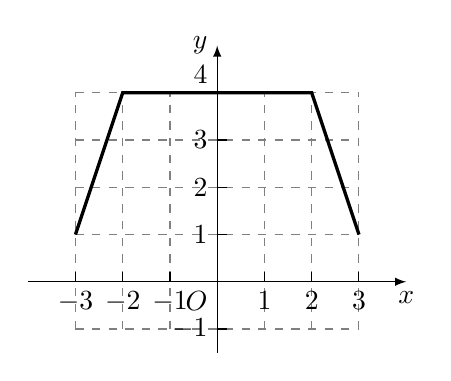
\begin{tikzpicture}[>=latex,scale = 0.6]
\foreach \i in {-3,-2,...,3}
{\draw [dashed, gray] (\i,-1) -- (\i,4);};
\foreach \i in {-1,0,...,4}
{\draw [dashed, gray] (-3,\i) -- (3,\i);};
\draw [->] (-4,0) -- (4,0) node [below] {$x$};
\draw [->] (0,-1.5) -- (0,5) node [left] {$y$};
\draw (0,0) node [below left] {$O$};
\draw [very thick] (-3,1) -- (-2,4) -- (2,4) -- (3,1);
\foreach \i in {-3,-2,-1,1,2,3}
{\draw (\i,0.2) -- (\i,0) node [below] {$\i$};};
\foreach \i in {-1,1,2,3}
{\draw (0.2,\i) -- (0,\i) node [left] {$\i$};};
\draw (0,4) node [above left] {$4$};
\end{tikzpicture}
\end{center}
\item 奇函数的图像是不是一定通过原点? 偶函数的图像是不是一定与$y$轴相交?  请说明理由.
\item 如图, 已知偶函数$y=f(x)$在$y$轴及$y$轴一侧的部分图像, 作出$y=f(x)$的大致图像.\\
(1) \begin{tikzpicture}[>=latex, samples = 200]
    \draw [->] (-3,0) -- (0,0) node [above left] {$O$} -- (3,0) node [below right] {$x$};
    \draw [->] (0,-1) -- (0,3) node [left] {$y$};
    \draw [domain = -3:0] plot (\x , {-\x * \x * \x / 8+ \x * \x /8 +\x});
    \end{tikzpicture}\\
(2) \begin{tikzpicture}[>=latex, samples = 200]
	\draw [->] (-3,0) -- (0,0) node [below left] {$O$} -- (3,0) node [below right] {$x$};
	\draw [->] (0,-1) -- (0,3) node [left] {$y$};
	\draw [domain = 0:3] plot (\x, {sin(\x * 60) * \x - 0.5});
	\end{tikzpicture}
\item 证明下列函数是奇函数:\\
(1) $y=2^x-2^{-x}$;\\
(2) $y=\log_2(1+x)-\log_2(1-x)$. 
\item 判断下列函数的奇偶性, 并说明理由:\\
(1) $y=|x|$;\\
(2) $y=\dfrac 1{1+x}-\dfrac 1{1-x}$;\\
(3) $y=x^3-x$, $x\in [-3, 3)$;\\
(4) $y=0$, $x\in [-1, 1]$.
\item 已知$a$是实数, 而定义在$\mathbf{R}$上的函数$y=f(x)$的表达式为$f(x)=|x-a|$.\\
(1) 是否存在实数$a$, 使得$y=f(x)$是奇函数? 说明理由;\\
(2) 是否存在实数$a$, 使得$y=f(x)$是偶函数? 说明理由. 
\item 小明说: ``如果当$x>0$时, 总有$f(x)>f(0)$, 那么函数$y=f(x)$在区间$[0, +\infty)$上是严格增函数.''他的说法是否正确? 说明理由.
\item 证明: 函数$y=\dfrac2{x^3}$在区间$(-\infty, 0)$上是严格减函数.
\item 构造一个二次函数, 使得它在区间$[-1, 1]$上是严格减函数, 并说明理由.
\item 根据下列函数$y=f(x)$的图像(包括端点), 分别指出这两个函数的单调区间, 以及在每一个单调区间上函数的单调性.\\
(1) \begin{tikzpicture}[>=latex]
    \draw [->] (-3.5,0) -- (0,0) node [below left] {$O$} -- (3.5,0) node [below right] {$x$};
    \draw [->] (0,-3) -- (0,3) node [left] {$y$};
    \draw [very thick] (-3,-1) -- (-2,-2) -- (-1,-1) -- (1,3) -- (2,1) -- (3,2);
    \foreach \i in {1,2,3}
    {\draw (\i,0) node [below] {$\i$};
        \draw (-\i,0) node [above] {$-\i$};}
    \draw [gray, dashed] (-3,0) -- (-3,-1) (-2,0) -- (-2,-2) (-1,0) --(-1,-1) (1,0)--(1,3) (2,0) -- (2,1) (3,0) -- (3,2);
    \end{tikzpicture}\\ 
(2) \begin{tikzpicture}[>=latex, samples = 200]
    \draw [->] (-3.5,0) -- (0,0) node [below left] {$O$} -- (3.5,0) node [below right] {$x$};
    \draw [->] (0,-3) -- (0,3) node [left] {$y$};
    \draw [domain = -pi:pi, very thick] plot (\x, {-2.5*sin(\x/pi*180)});
    \draw [gray, dashed] (-pi/2,0) --+ (0,2.5) (pi/2,0) --+ (0,-2.5);
    \draw (-pi,0) node [below] {$-\pi$} (-pi/2,0) node [below] {$-\dfrac{\pi}{2}$} (pi/2,0) node [above] {$\dfrac{\pi}{2}$} (pi,0) node [above] {$\pi$};
    \end{tikzpicture}
\item 判断函数$y=|x+1|$, $x\in [-2, 2]$的单调性, 并求出其单调区间.
\item 设$y=f(x)$是奇函数, 且它在区间$(-3, 0]$上是严格增函数.\\
(1) 求证: 它在区间$[0, 3)$上是严格增函数;\\
(2) $y=f(x)$是否在区间$(-3, 3)$上是严格增函数? 说明理由.
\item 求函数$y=(\dfrac 12)^x$, $x\in [1, 3]$的最大值与最小值.
\item 求下列函数的最大值与最小值:\\
(1) $y=1-x^2$;\\
(2) $y=1-x^2$, $x\in [-1, 2]$;\\
(3) $y=2x^2-8x$;\\
(4) $y=2x^2-8x$, $x\in [0, 1]$.
\item 已知$a>-2$, 求函数$y=x^2+1$, $x\in [-2, a]$的最大值.
\item 已知一等腰三角形的周长为$12\text{cm}$, 试将该三角形的腰长$y$(单位: $\text{cm}$)表示为底边长$x$(单位: $\text{cm}$)的函数.
\item 如图, 在平面直角坐标系的第一象限内, $\triangle OAB$是边长为$2$的等边三角形. 用直线$l: x=t$($0<t<2$)截这个三角形, 记截得的靠近$y$轴的部分的面积为$S$. 试将$S$表示为$t$的函数.
\begin{center}
    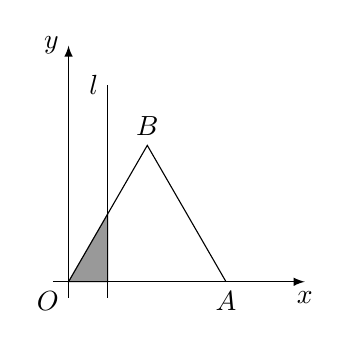
\begin{tikzpicture}[>=latex]
        \filldraw [gray!80] (0,0) -- (60:1) -- (0.5,0) -- cycle;
        \draw [->] (-0.2,0) -- (3,0) node [below] {$x$};
        \draw [->] (0,-0.2) -- (0,3) node [left] {$y$};
        \draw (0,0) -- (60:2) node [above] {$B$} -- (2,0) node [below] {$A$};
        \draw (0,0) node [below left] {$O$};
        \draw (0.5,-0.2) -- (0.5,2.5) node [left] {$l$};
    \end{tikzpicture}
\end{center}
\item 某商场购物优惠活动如下: 一次购物总额不超过$500$元的不予优惠; 一次购物总额超过$500$元但不超过$1000$元的, 按标价给予$9$折优惠; 一次购物总额超过$1000$元的, 其中的$1000$元按上述标准给予优惠, 而超过$1000$元的部分给予$7$折优惠. 设某位顾客一次购物总额为$x$元, 而优惠后实际付款额为$y$元. 试写出$y$关于$x$的函数关系.
\item 利用函数与不等式的关系, 在$a<0$时, 求解实系数一元二次不等式$ax^2+bx+c\le 0$.
\item 用函数的观点解不等式: $2^x+\log_2x>2$.
\item 对于在区间$[a, b]$上的图像是一段连续曲线的函数$y=f(x)$, 如果$f(a)\cdot f(b)>0$, 那么是否该函数在区间$(a, b)$上一定无零点? 说明理由.
\item 已知函数$y=2x^3-3x^2-18x+28$在区间$(1, 2)$上有且仅有一个零点. 试用二分法求出该零点的近似值. (结果精确到$0.1$)
\item 求函数$y=x^2+2x$, $x\in [0, +\infty)$的反函数的定义域.
\item 求下列函数的反函数:\\
(1) $y=3x+2$;\\
(2) $y=-\dfrac 3x$;\\
(3) $y=x^2$, $x\in (-\infty, 0]$;\\
(4) $y=\sqrt x+1$.
\item 判断函数$y=\begin{cases}x, & -1\le x\le 0, \\ 1-x, & 0<x<1\end{cases}$是否存在反函数. 若存在反函数, 求出它的反
函数; 若不存在反函数, 说明理由. 
\item 定义在$\mathbf{R}$上的偶函数存在反函数吗? 说明理由.
\item 下列各图中, 存在反函数的函数$y=f(x)$的图像只可能是\bracket{20}.
\fourch{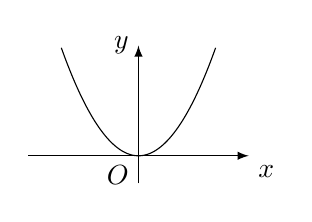
\begin{tikzpicture}[>=latex,samples=200,scale =0.7]
\draw [->] (-2,0) -- (0,0) node [below left] {$O$} -- (2,0) node [below right] {$x$};
\draw [->] (0,-0.5) -- (0,2) node [left] {$y$};
\draw [domain=-1.4:1.4] plot (\x, \x * \x);
\end{tikzpicture}}{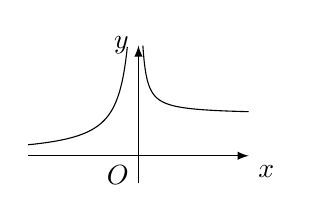
\begin{tikzpicture}[>=latex,samples=200,scale =0.7]
\draw [->] (-2,0) -- (0,0) node [below left] {$O$} -- (2,0) node [below right] {$x$};
\draw [->] (0,-0.5) -- (0,2) node [left] {$y$};
\draw [domain=-2:-0.2] plot (\x, {-0.4/ \x});
\draw [domain=0.08:2] plot (\x, {0.1/\x+0.75});
\end{tikzpicture}}{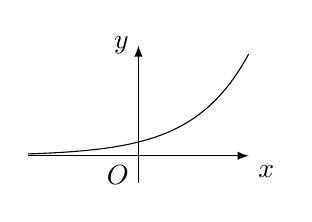
\begin{tikzpicture}[>=latex,samples=200,scale =0.7]
\draw [->] (-2,0) -- (0,0) node [below left] {$O$} -- (2,0) node [below right] {$x$};
\draw [->] (0,-0.5) -- (0,2) node [left] {$y$};
\draw [domain=-2:2] plot (\x, {exp(\x)/4});
\end{tikzpicture}}{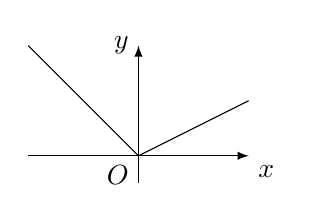
\begin{tikzpicture}[>=latex,samples=200,scale =0.7]
\draw [->] (-2,0) -- (0,0) node [below left] {$O$} -- (2,0) node [below right] {$x$};
\draw [->] (0,-0.5) -- (0,2) node [left] {$y$};
\draw (-2,2) -- (0,0) -- (2,1);
\end{tikzpicture}}
\item 已知函数$y=f(x)$, $x\in D$存在反函数$y=f^{-1}(x)$, $x\in f(D)$. 函数$y=f(x+1)$与$y=f^{-1}(x+1)$是否一定互为反函数? 说明理由. 

\end{enumerate}

\end{document}